\section{RANSOM: System Design and Implementation}

\subsection{Architecture}

\annie{discuss architecture overview here.}

\begin{figure}[t]
\centering
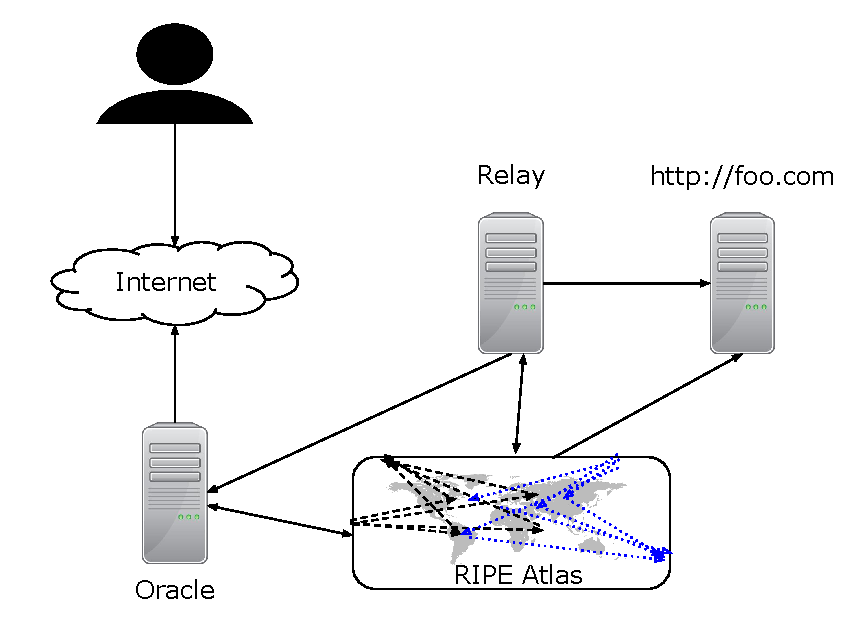
\includegraphics[width=.5\textwidth]{architecture}
\caption{RANSOM architecture.}
\label{fig:arch}
\end{figure}

\subsection{Goals}

{\bf Foreign Country Avoidance.}

{\bf Usability.}

{\bf Scalability.}

{\bf Non-goals.}  \annie{Discuss anonymity and domestic surveillance}

\subsection{Calculating Paths}

{\bf Client to Relay Paths.}

{\bf Relay to Client Paths.}

{\bf Relay to Server Paths.}

{\bf Client to Server Paths.}

\annie{Discuss re-computation (and include how many country-level paths change per hour/per 2 hours on average, selection of servers/domains, justify argument against traffic analysis because we have 3/4 paths}

\subsection{Multiplexing Between Relays}

\annie{Discuss .pac file and characteristics and generation and re-generation}

\subsection{Adding and Removing Relays}

{\bf Adding Relays.}

{\bf Removing Relays.}

\subsection{Additional Features}

{\bf Privacy-preserving features at proxy.}

{\bf Load balancing and congestion control.}
